% TODO Figuren uitzoeken
\chapter{Functioneel ontwerp SOUP API}\label{ch:impl soup api}
De SOUP-API is de centrale module voor het systeem dat verantwoordelijk is voor het periodiek scannen van de projecten, het parsen van de rapporten die uit de analyses komt en het beschikbaar maken van de data die in de datbase is opgeslagen. In dit hoofdstuk wordt functioneel ingegaan op de werking van dit deel van de applicatie en zijn de drie sub-modulen die ieders een deel van deze taken op zich neemt beschreven. Eerst zal de algmene functionaliteit van de API behandeld worden om vervolgens de iets grotere functies zoals het parsen van de SCA rapportage en het regelen van het periodieke analyse systeem te behandelen.


\section{API}\label{sec:api2}
Centraal in de SOUP-API staat de API welke verantwoordelijk is om de data die door de beide Engines, beschreven in het hoofdstuk Architectuur, te verwerken en in goede banen te leiden. De API zal de Controller, Service en Repository structuur aanhouden.

Om de data die in het datamodel (zie figuur~\ref{fig:SOUP-SoupApiDm [CHECKEN]} in het vorige hoofdstuk) gedefineerd is te bedienen is er gekozen voor een model, service, repository architectuur. Voor iedere entiteit in het datamodel is een case class geschreven met daarbij een companionobject wat direct de mogelijkheid biedt om deze classes om te zetten in JSON voor opslag in de database en verzenden van en naar de API. De business logica is belegt in services, waarbij er voor iedere entitiet een service is aangemaakt die mutaties op deze entiteiten mogelijk maakt, waarbij naast de standaard CRUD acties ook relaties tussen de entiteiten kunnen worden gemaakt. De repository maakt het vervolgens mogelijk om data van en naar de database te versturen.

\begin{figure}[bth]
    \myfloatalign
    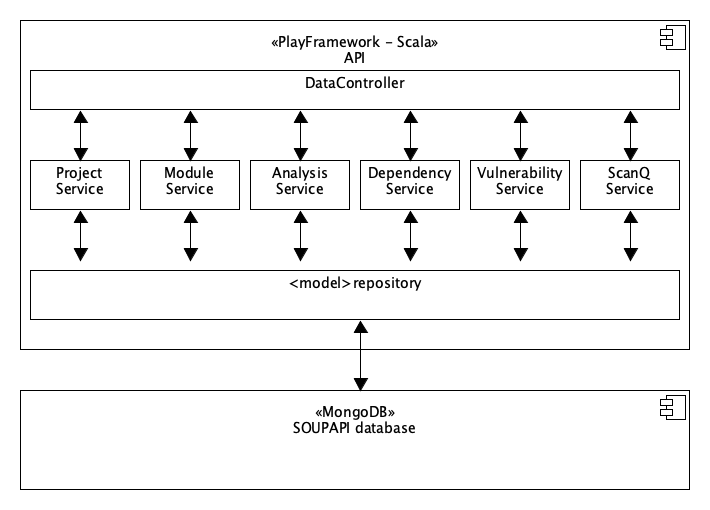
\includegraphics[width=12cm]{gfx/umlet/exports/API-ComponentsDiagram}
    \caption{API components Controllers, Services en Repositories}
    \label{fig:API components}
\end{figure}


\subsection{Controllers}\label{subsec:controllers}
Voor iedere entiteit dat belegt is in het interne datamodel (figuur~\ref{fig:SOUP-SoupApiDm [CHECKEN]} worden algemene REST endpoints aangemaakt die bewerkingen op data beschikbaar maken waar dit gewenst en mogelijk is.
\subsubsection{DataController}
Controller voor het beheer van de data in de database. De REST endpoints maken het mogelijk om data te bewerken. In de secties hieronder kan [Entiteit] worden gelezen als alle Entiteiten in het interne datamodel, met als uitzondering Dependencies en Vulnerabilities. Dit gezien deze laatste twee gegenereert worden door de raportage en bewerking van buitenaf niet gewenst is in verband met de integriteit van deze data.
\subsubsection*{Create}
Bij een create dient het ID van de aangemaakte entiteit te worden teruggeven aan de client.

\textbf{POST: /data/[Entiteit]/} maakt een enititeit aan volgens de in de body meegegeven DTO.

\subsubsection*{Read}
Als er een read actie wordt aangeroepen kan alleen de entiteit op zichzelf worden weergegegeven of een gedetaileerde weergave hiervan inclusief gerelateerde entiteiten.

\textbf{GET: /data/[Entiteit]/?detail=[boolean]} haalt alle mogelijke records op van de betreffende entiteit. Door detail op true te zetten komen ook alle sub entiteiten mee met de return body.

\textbf{GET: /data/[Entiteit]/?detail="[boolean]"\&attr="[attribuut]\&value="[value]} haalt een enkele entiteit op van een enkele record op basis van het meegegeven attribuut en de value van dat attribuut. Als er bijvoorbeeld een enkel project moet worden opgehaald op basis van de naam is de volgende HTTP POST Call op "/data/project/?detail=true&attr="name"&value="groeigids$"$ de manier om het project groeigids op te halen.

\subsubsection*{Update}
\textbf{PUT: /data/[Entiteit]/?attr="[Attribuut]\&value="[value]"} update een door de attribuut en value geselecteerde record met de meegegeven body.
\subsubsection*{Delete}
\textbf{DELETE: /data/[Entitiet]/?attr="[Attribuut]\&value="[value]"} verwijderd een record dat gevonden wordt middels het meegegeven attribuut en de bijbehorende value.


\subsubsection{UploadController}
De uploadController fungeerd als gateway waar rapporten naar toe kunnen worden geupload. Er kunnen vanuit twee processen binnen de SOUP applicatie rapporten worden geupload. Voor beide is een eigen endpoint voorzien:

\textbf{POST: /upload/jenkins} geeft een endpoint met de mogelijkheid om meerdere bestanden te uploaden. Als eerste is er het SCA rapport met daarin de resultaten van de eerste analyse. Bij de analyse middels Jenkins worden ook de dependency files meegezonden om op die manier het systeem up-to-date te houden. Als laatst wordt er een JSON bestand meegestuurt met daarin de meta gegevens over het project.

\begin{figure}[bth]
    \myfloatalign
    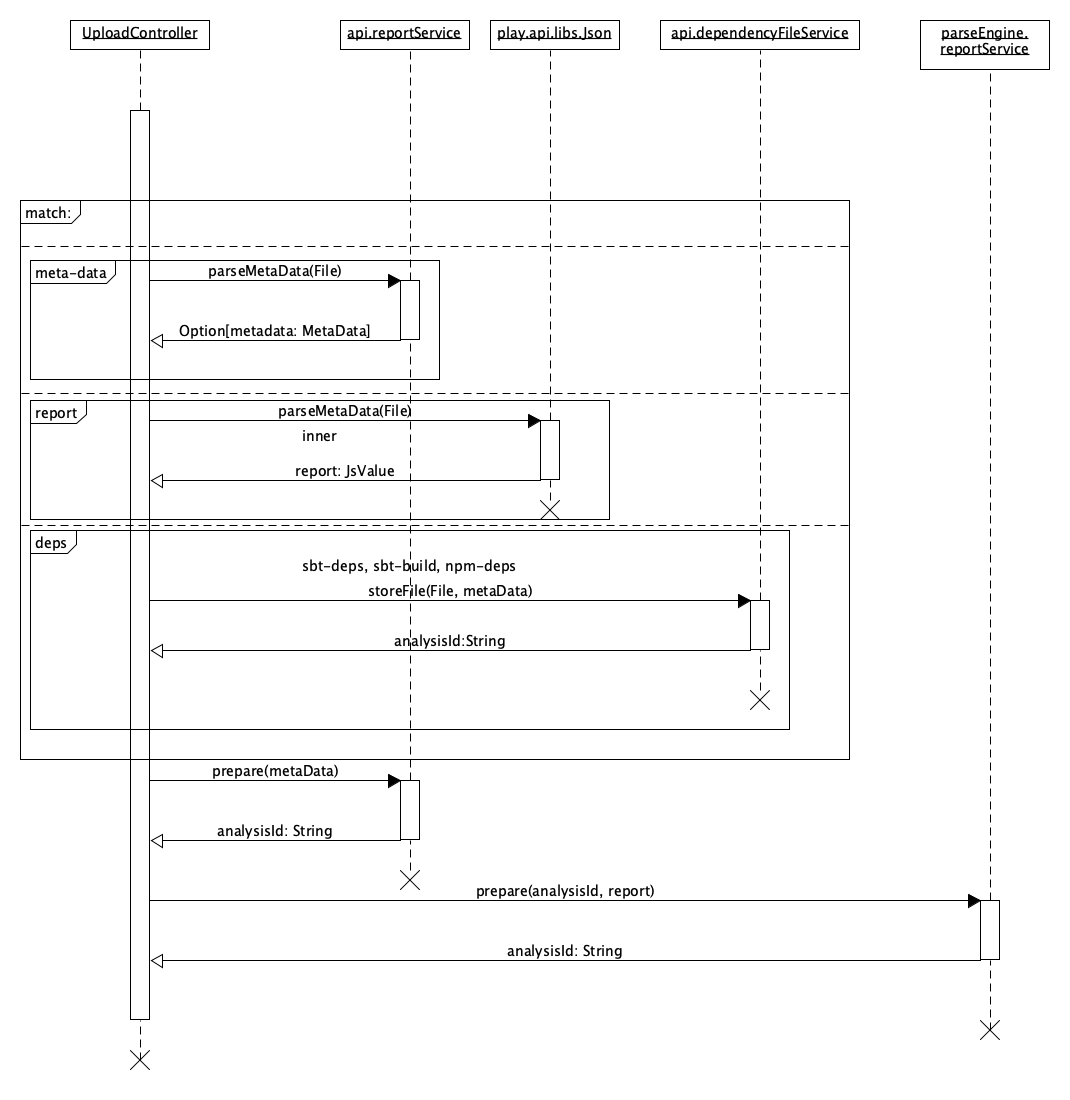
\includegraphics[width=12cm]{gfx/umlet/exports/SequploadController-Jenkins}
    \caption{Sequence UploadController Jenkins endpoint}
    \label{fig:SequenceUploadReportJenkins}
\end{figure}

\textbf{POST: /upload/pae} dit endpoint geeft alleen de mogelijkheid om het SCA rapport en de meta data up te loaden welke vervolgens kunnen worden verwerkt door de SOUP-API. Gezien er in de Analysis Engine geen veranderingen in de dependencies zijn hoeven deze dan ook niet te worden meegezonden.

\begin{figure}[bth]
    \myfloatalign
    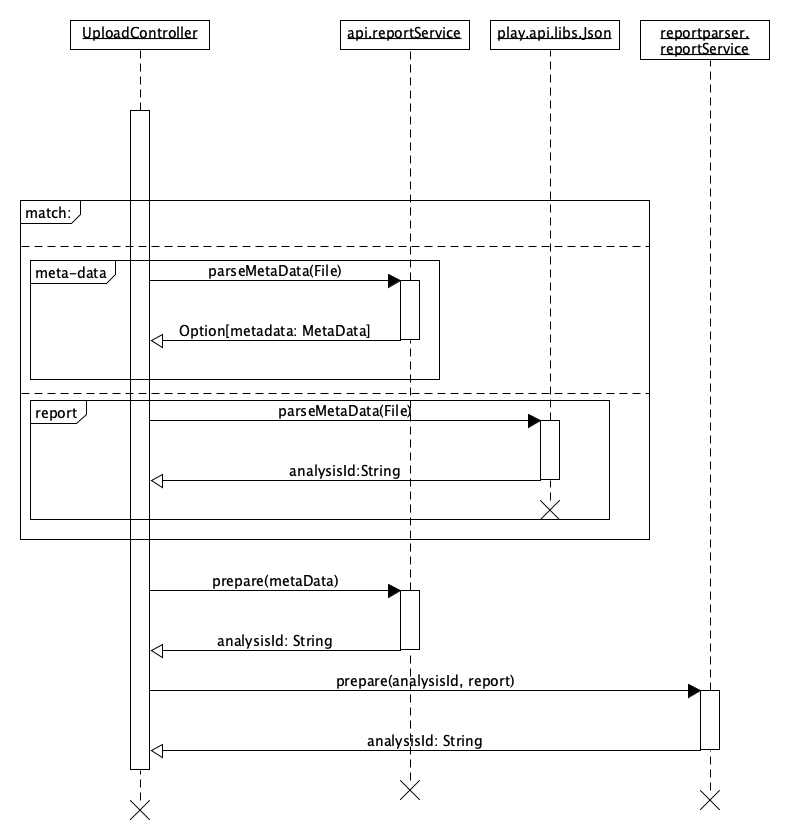
\includegraphics[width=12cm]{gfx/umlet/exports/SequploadController-pae}
    \caption{Sequence UploadController Periodic Analysis Engine endpoint}
    \label{fig:SequenceUploadReportpaet}
\end{figure}

In beide gevallen worden er bestanden naar de uploadcontroller verstuurt. De bestanden zijn onderdeel van de body en worden voorzien van een key. Hieronder is te zien welke bestanden de controller kan verwachten en met welke key deze geidentificeert kan worden. Alleen dependencybestanden worden verstuurt naar de \texttt{/upload/jenkins/} endpoint.

\begin{tabular}{lll}
    \textbf{key} & \textbf{Type} & \textbf{bestand} \\
    report & JSON & het SCA Rapport \\
    meta-data & JSON & Meta Data over de analyse uit jenkins \\
    sbt-deps & scala source & dependencydeclarite uit SBT project \\
    sbt-build & build.sbt  & build file van SBT project\\
    npm-deps & JSON & package-lock.json \\
    dockerFile & dockerFile & base image dockerfile
\end{tabular} \\
Zoals te zien is in figuur ~\ref{fig:SequenceUploadReportJenkins} en \ref{fig:SequenceUploadReportpaet} wordt er direct in de controller de bestanden omgezet naar data die binnen de SOUPAPI gebruikt kan worden. De dependency en docker bestanden worden middels de DependencyFileService opgeslagen in de fileSystem en de database, de metaData wordt omgezet in een object van de case class MetaData zodat de attributen makkelijk te bereiken zijn. Het rapport wordt omgezet naar JSON zodat deze door de ReportParseEngine kan worden verwerkt. Als alle bestanden zijn verwerkt wordt er een analyse aangemaakt welke door de ReportParseEngine kan worden gebruikt voor het opslaan van het rapport.

\subsection{Services}\label{subsec:Services}
Voor de business logica is er een services laag die de verschillende processen in de SOUP-API belegt. In principe zijn er twee hoofd typen processen: De verwerking van rapportage over kwetsbaarheden en de services die de bewerkingen op data regelen.
De reportservice zorgt voor de verbinding tussen de API en de ReportParseService. Daarnaast biedt het de mogelijkheid om in de toekomst het volledige rapport in te kunnen zien.
De Data Services zijn een tussenlaag tussen de dataControllers en de Datarepositories die het mogelijk maken om entiteiten toe te voegen en relaties tussen entiteiten te leggen. Het biedt ook de mogelijkheid om records op te halen op basis van deze relaties.

\subsection{Repositories}\label{subsec:repositories}
Net als bij de services is voor iedere Entiteit in het datamodel een eigen repository geschreven die de interactie met de database mogelijk maakt. In elke repository zijn de basis bewerkingen belegt. Voor iedere entiteit zijn onderstaande functies geschreven:

\begin{tabular}{ll}
    \textbf{function} & \textbf{Returns}\\
    create(e: Entity) & Future[Boolean] \\
    createMany(deps: Seq[Entity])& Future[Boolean]\\
    findOneById(id: String) & Future[Option[Entity]]\\
    findOneByName(name: String) & Future[Option[Entity]]\\
    findAll() & Future[Seq[Entity]] \\
    update(id: String, e: Entity) & Future[Boolean]\\
    delete(id: String) & Future[Boolean] \\
\end{tabular} \\

%https://stackoverflow.com/questions/70513344/scala-generic-repository-class-for-reactive-mongo-repositoryalpakka-needed-c

\subsubsection{DTO's}
Omdat niet altijd het gehele object van en naar de client wordt verstuurt worden er DTO's aangemaakt. Deze kunnen worden gebruikt als afspraak tussen de backend en de client. Een voorbeeld van een DTO is de volgende:

In de Jenkins upload controller wordt er naast een rapport ook metadata verstuurt middels een JSON bestand. In de backend is de volgende case class gedefineerd met de benodigde gegevens:
\begin{lstlisting}[caption={case class MetaData in MetaData.scala},label=lst:metdataScala]

package domain.dtos
import play.api.libs.json.{Json, OFormat}

case class MetaData(
                     projectName: String,
                     moduleName: String,
                     platform: String,
                     runtimeVersion: String,
                     buildToolVersion: String,
                     tool: String,
                     gitHash: String,
                     jenkinsBuildNr: String
                   )

object MetaData {

  implicit val projectFormat: OFormat[MetaData] = Json.format[MetaData]
}

\end{lstlisting}
\newpage
Wat vervolgens in de volgende JSON resulteert:
\begin{lstlisting}[caption={metadata JSon object behorende bij de case class}, label={lst:metadatajson}]
{
  "projectName": "testProject",
  "moduleName": "backend",
  "platform": "sbt",
  "runtimeVersion": "2.13.6",
  "buildToolVersion": "1.5.0",
  "tool": "owasp",
  "gitHash": "6cf71dd74241e6292db69368f1d4f6d990b3f03s",
  "jenkinsBuildNr": "42"
}
\end{lstlisting}
\subsection{Algehele CRUD functionaliteit}\label{subsec:algehele-crud-functionaliteit}
In deze hele sectie is het de entiteit project als voorbeeld genomen om de verschillende bewerkingen in het systeem weer te geven
\subsubsection*{Create}
In figuur ~\ref{fig:seqdiagcreateProj} is te zien hoe een project aangemaakt wordt in de database door vanuit de datacontroller een Project Object naar de ProjectService te sturen welke het vervolgens naar de repository verstuurt de de communicatie met de database verzorgt. De repository geeft Future[WriteResult]\footnote{Een Future kan gezien worden als een async promise uit JavaScript} terug. Een WriteResult is een object welke uit de ReactiveMongo Bibliotheek wordt terug gegeven in dit object is metadata over de actie op de database. De service zal nagaan of de actie gelukt is en op het moment dat dit zo is een Option[Project]\footnote{Een Option kan een instantie van een object bevatten of een None. Waarmee in een latere moment de keuze kan worden gemaakt wat er mee te doen. dit geeft de mogelijkheid om alle foutafhandeling op een zelfde niveau te regelen wat de structuut van de applicatie ten goede brengt.} terug geven. De Controller kan op basis van de option aangeven of de actie voltooid en gelukt is of dat er ergens iets fout is gegaan.
\begin{figure}[h]
    \myfloatalign
    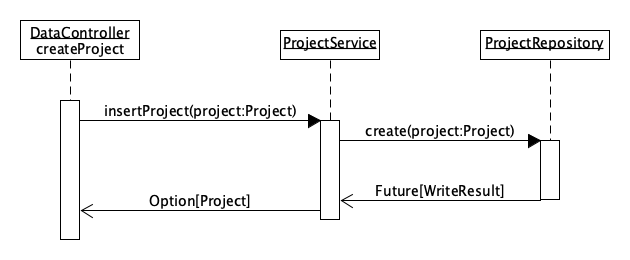
\includegraphics[width=10cm]{gfx/umlet/exports/CRUD-CreateProject}
    \caption{Sequence Diagram Create Project }
    \label{fig:seqdiagcreateProj}
\end{figure}



\subsubsection*{Find(One/All)}
In figuur ~\ref{fig:seqdiagFindProj} is te zien hoe een project gevonden kan worden middels een in de parameter meegegeven attribuut en value voor dit attribuut. ( zie sectie ~\ref{subsec:controllers}) de projectService roept op basis van het meegegeven attribuut de juiste functie aan in de projectRepository. Het resultaat is een Future[Option[Project]] welke door de service wordt afgehandeld en deze als een Option[Project] naar de controller wordt gestuurd.
\begin{figure}[h]
    \myfloatalign
    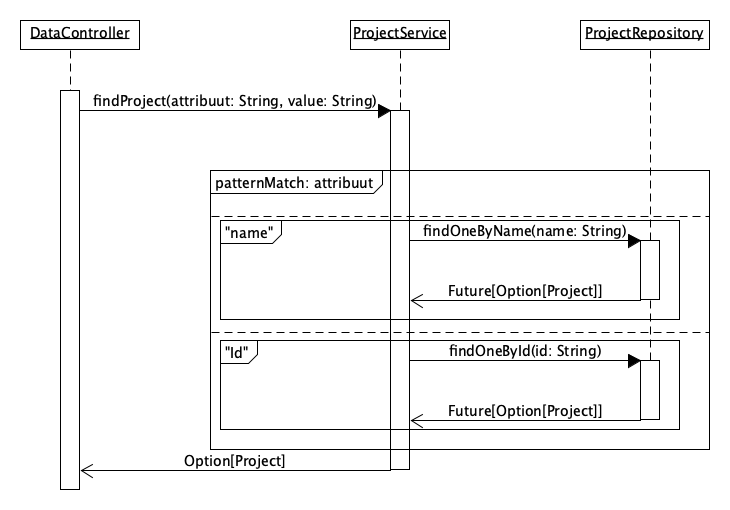
\includegraphics[width=10cm]{gfx/umlet/exports/CRUD-FindProject}
    \caption{Sequence Diagram FindOne Project }
    \label{fig:seqdiagFindProj}
\end{figure}
\subsubsection*{Update}Schema maken
In figuur ~\ref{fig:seqdiagUpdateProj} is te zien hoe een project kan worden geupdate. Het maakt in weze gebruik van hetzelfde mechanisma als de findOne functionaliteit als hierboven. Echter wordt er een project object meegezonden met daarin de nieuwe gegevens
\begin{figure}[h]
    \myfloatalign
    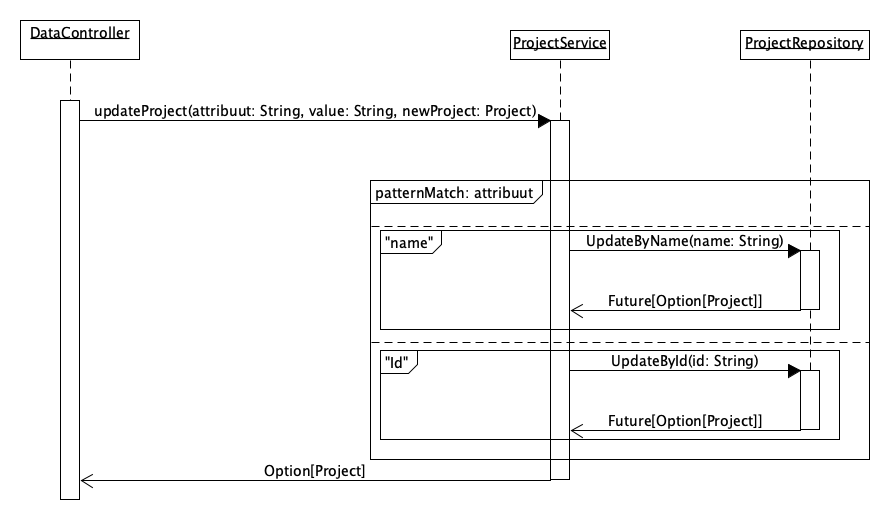
\includegraphics[width=10cm]{gfx/umlet/exports/CRUD-UpdateProject}
    \caption{Sequence Diagram Update Project }
    \label{fig:seqdiagUpdateProj}
\end{figure}
\subsubsection*{Delete}
In figuur ~\ref{fig:seqdiagDeleteProj} is te zien hoe een project wordt verwidjerd. Door wederom het zelfde mechanisme van attribuut en value te gebruiken zoals beschreven in de find sectie hierboven kan een te verwidjeren object geselcteerd worden en vervolgens verwijderd
\begin{figure}[h]
    \myfloatalign
    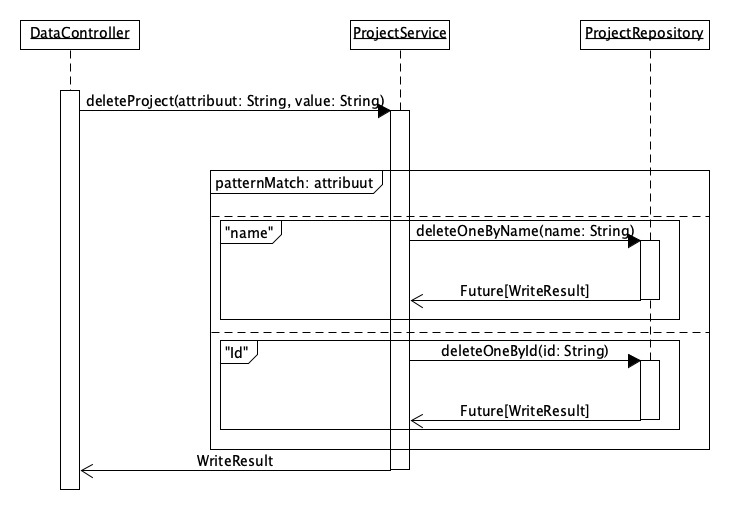
\includegraphics[width=10cm]{gfx/umlet/exports/CRUD-DeleteProject}
    \caption{Sequence Diagram Delete Project }
    \label{fig:seqdiagDeleteProj}
\end{figure}

\subsection{Toevoegen van entiteit A aan entiteit B}\label{subsec:toevoegen-van-entiteit-a-aan-entiteit-b}
Als voorbeeld wordt in deze sectie het toevoegen van een module aan een project getoont. Het geeft weer hoe de relaties tussen verschillende entiteiten worden gedaan. In figuur~\ref{fig:seqdiagModToProj} is te zien dat er een call
gedaan wordt vanuit de ReportService waarbij de Id's van zowel het project als de module wordt meegegeven. Als eerst wordt er een project opgehaald door middel van het ID. De module wordt toegevoegd aan dit project ( nadat er gekeken is of het project deze module nog niet heeft) en vervolgende wordt de repository aangeroepen om het project te updaten.
\begin{figure}[h]
    \myfloatalign
    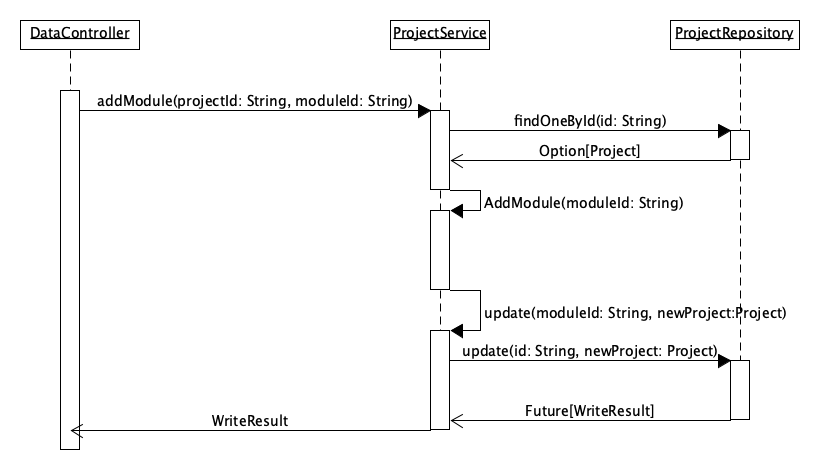
\includegraphics[width=10cm]{gfx/umlet/exports/Relation-ModuleToProject}
    \caption{Sequence Diagram Add Module to Project }
    \label{fig:seqdiagModToProj}
\end{figure}

\newpage
\section{Report Parse Engine}\label{sec:report-parse-engine}
De ReportParseEngine is verantwoordelijk voor het omzetten van een rapport dat gegenereerd wordt door een Software Composition Analysis Tool naar het interne datamodel. Het feit dat er veel tools zijn die allemaal de mogelijkheid bieden om projecten te analyseren op kwetsbaarheden en hier een rapport over uit te brengen geeft al aan dat de ReportParseEngine in staat moet zijn om met verschillende rapporten van verschillende tools om te moeten kunnen gaan. Om dit mogelijk te maken is er gekozen voor een modulaire opzet waarbij er verschillende parsers geschreven kunnen worden die de rapporten kunnen omzetten. Deze Modulaire opzet is te zien in figuur~\ref{fig:ReportParseComponents} waarbij de $"$[FUTURE]Parser$"$ een placeholder is voor elke parser die in de toekomst moet worden toegevoegd om meerdere tools te kunnen ondersteunen.
\begin{figure}[bth]
    \myfloatalign
    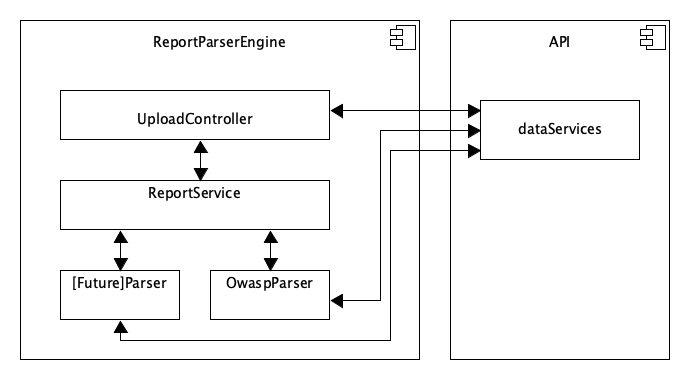
\includegraphics[width=12cm]{gfx/umlet/exports/ReportParserComponents}
    \caption{ReportParseEngine Components}
    \label{fig:ReportParseComponents}
\end{figure}


\subsection{ParserService}\label{subsec:reportservice}
De ParserService ontvangt van de uploadController beschreven hierboven naast het rapport in JSON, de metaData ook een analyseId. Dat laatste wordt gebruikt om de dependency/vulnerability informatie uit het rapport toe te voegen aan de analyse. in de metaData staat welke tool er gebruikt is voor het opzetten van het rapport en kan daarmee gebruikt worden om de juiste parser te selecteren voor het omzetten van het rapport.

\begin{figure}[bth]
    \myfloatalign
    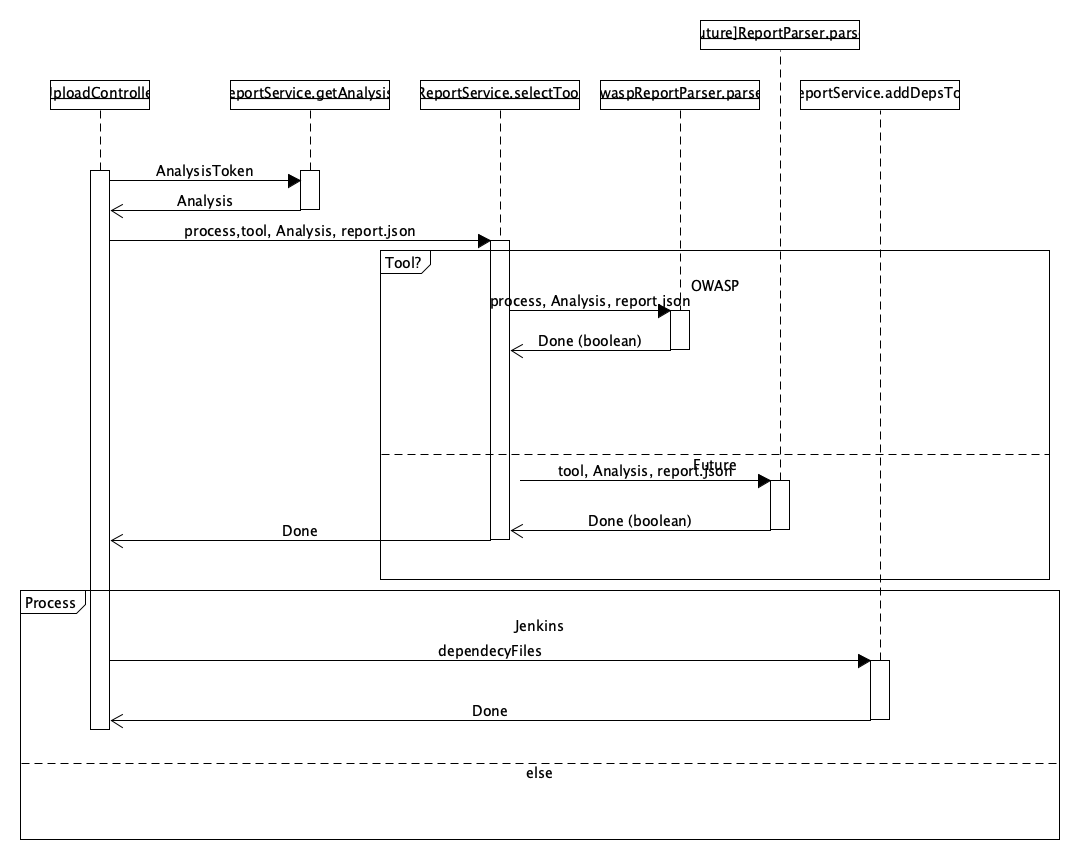
\includegraphics[width=14cm]{gfx/umlet/exports/SeqProcessPayload}
    \caption{Sequence diagram Proces Payload}
    \label{fig:ProcesPayload}
\end{figure}

\subsection{OWASP Parser}\label{subsec:owasp-parser}
De OWASP parser is verantwoordelijk voor het omzetten van binnengekomen OWASP data in JSON naar data in de database waarbij de onderlinge relaties blijven bestaan.
Omdat in een eerdere stap er al een analyse is aangemaakt dienen alleen nog de dependencies en de bijbehorende vulnerabilities te worden toegevoegd. De methode hiervoor is te zien in figuur ~\ref{fig:seqReportParse}
De parser dient dan ook te moeten weten welke analyse er is aangemaakt Deze wordt middels een ID meegegeven alsook het OWASP rapport. De Parser zet de gevonden dependencies en kwetsbaarheden om naar het de intern geldende entiteiten en voegt deze middels de dataServices toe aan de database.

\begin{figure}[bth]
    \myfloatalign
    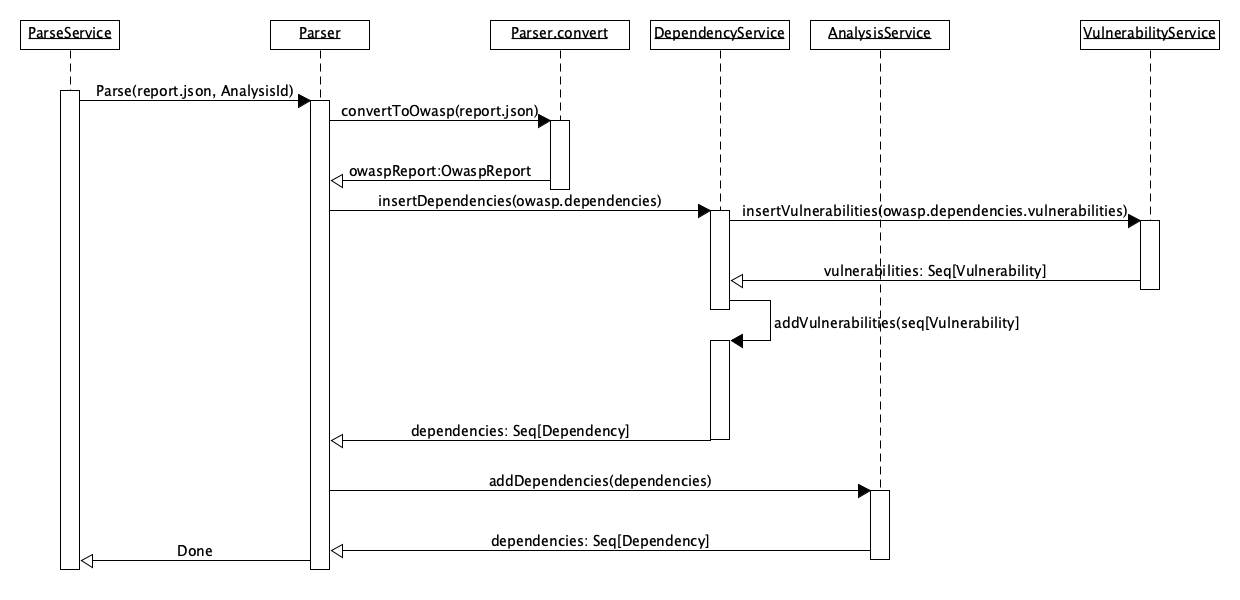
\includegraphics[width=10cm]{gfx/umlet/exports/Seq-ParseReport}
    \caption{Sequence Diagram verwerken dependencies en vulnerabilites}
    \label{fig:seqReportParse}
\end{figure}


\subsection{$"$[Future]Parser$"$}\label{subsec:$"$[future]parser$"$}
De $"$[Future]Parser$"$ zal in basis gelijk zijn als de parser voor de OWASP tool die hierboven worden beschreven. Echter zal de daadwerklijke omzetting veranderen. Om deze reden moet er voor iedere tool een eigen datamodel worden gedifineerd waarmee er objecten kunnen worden gemaakt van deze Data. Waarbij er vervolgens middels deze objecten naar het interne datamodel worden gewerkt.

\clearpage


%TODO: Nog even goed over nadenken.....
\section{Periodic Analysis Engine}\label{sec:periodiek-analysis-engine}
De Periodic Analysis is verantwoordelijk voor het uitvoeren van analyses op de voor de SOUP-API bekende projecten/modulen. Hier voor maakt het gebruik van een omgeving die in sectie ~\ref{sec:analysis-environment} wordt beschreven. Om deze omgeving aan te sturen zijn er een aantal componenten nodig die in figuur~\ref{fig:paeComps} te zien zijn. Een tweetal CronJobs welke op gezete tijden een POST request maakt naar de Analysis Engine triggeren of wel een start of een stop commando. Deze commando's worden door de controller uitgevoerd. De controller is ook verantwoordelijk voor het verdere uitvoeren van de taken. die elk hieronder beschreven zullen worden. De beschreven service voorziet de controller van de benodigde data vanuit de API en de ScanQ. Dat laatste is een database tabel dat los staat van alle andere tabellen en houd de analyses bij die er gedaan moetene worden.
\begin{figure}[bth]
    \myfloatalign
    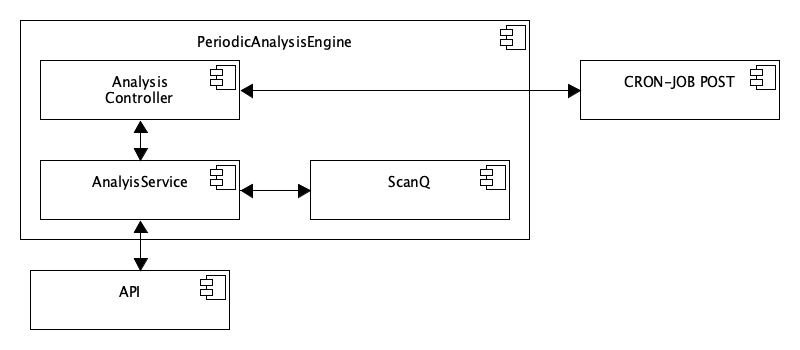
\includegraphics[width=10cm]{gfx/umlet/exports/PeriodicAnalyisEngineComponents}
    \caption{Componenten in de periodic Analysis Engine}
    \label{fig:paeComps}
\end{figure}
\begin{figure}[bth]
    \myfloatalign
    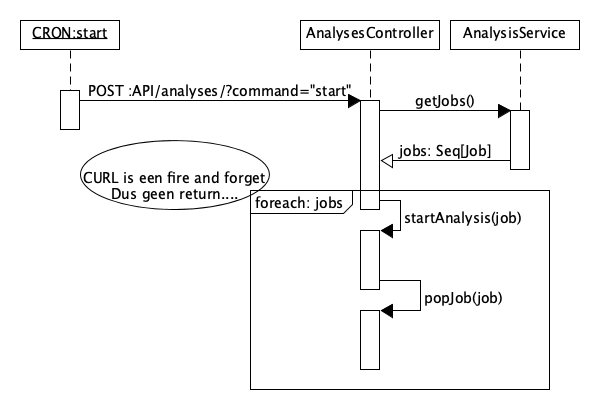
\includegraphics[width=10cm]{gfx/umlet/exports/PAE-jobssequence}
    \caption{Componenten in de periodic Analysis Engine}
    \label{fig:jobSeq}
\end{figure}

In figuur~\ref{fig:jobSeq} is te zien hoe de controller de job afhandeld na het ontvangen van een start commando.
\begin{enumerate}
    \item Een \textbf{CRON Job} triggered de controller door middel van een Start commando.
    \item Vervolgens wordt er in de \textbf{ScanQ} gekeken of er analyses zijn die zouden moeten gebeuren deze worden in een worklist gezet voor deze sessie.
    \item De \textbf{Analysis Controller} werkt de worklist af. Door de analyses te starten.
    \item Op het moment dat de analyse klaar is en opgeslagen in de database zal deze uit de worklist gehaald worden en een nieuwe datum op basis van de gekozen periode opnieuw in de \textbf{ScanQ} zetten door middel van de popJob functie.
    \item Dit proces blijft doorgaan tot er een \textbf{CRON Job} wordt verstuurt wat het proces stopt. De workList wordt leeg gemaakt waardoor de laatste analyse waar nog aan gewerkt wordt afgemaakt.
\end{enumerate}

Het stop commando haalt de worklist leeg zodat de loop eindigd en zo het proces stopt.

\subsection{CRON Jobs}\label{subsec:cron-jobs}
Er zijn een tweetal CRON Jobs nodig die er voor zorgen dat de analyser engine wordt gestart en gestopt:

\texttt{00 20 * * 5 curl -X POST http:/[souapi]/analyser/?command="start" >/dev/null 2>\&1} zorgt voor het starten van de engine op zaterdag om 20:00 door een post te doen naar de SOUP-API met het commando start.

\texttt{59 23 * * 5 curl -X POST http:/[souapi]/analyser/?command="stop" >/dev/null 2>\&1} zorgt voor het stoppen van de engine op zaterdag om 23:59 door een POST te doen naar de SOUP-API met het commando stop

Er kunnen nartuurlijk meer dagen worden toegevoegd waarin er in de avond wordt geanalyseerd. In basis zijn de commando's het zelfde. echter veranderd de dag van de week.

\subsection{AnalysisController}\label{subsec:analysiscontroller}
Naast het starten van de analyses is de controller ook verantwoordelijk voor het aanmaken van de analyseContainers en daarin het uitvoeren van de Analyse.
\begin{figure}[bth]
    \myfloatalign
    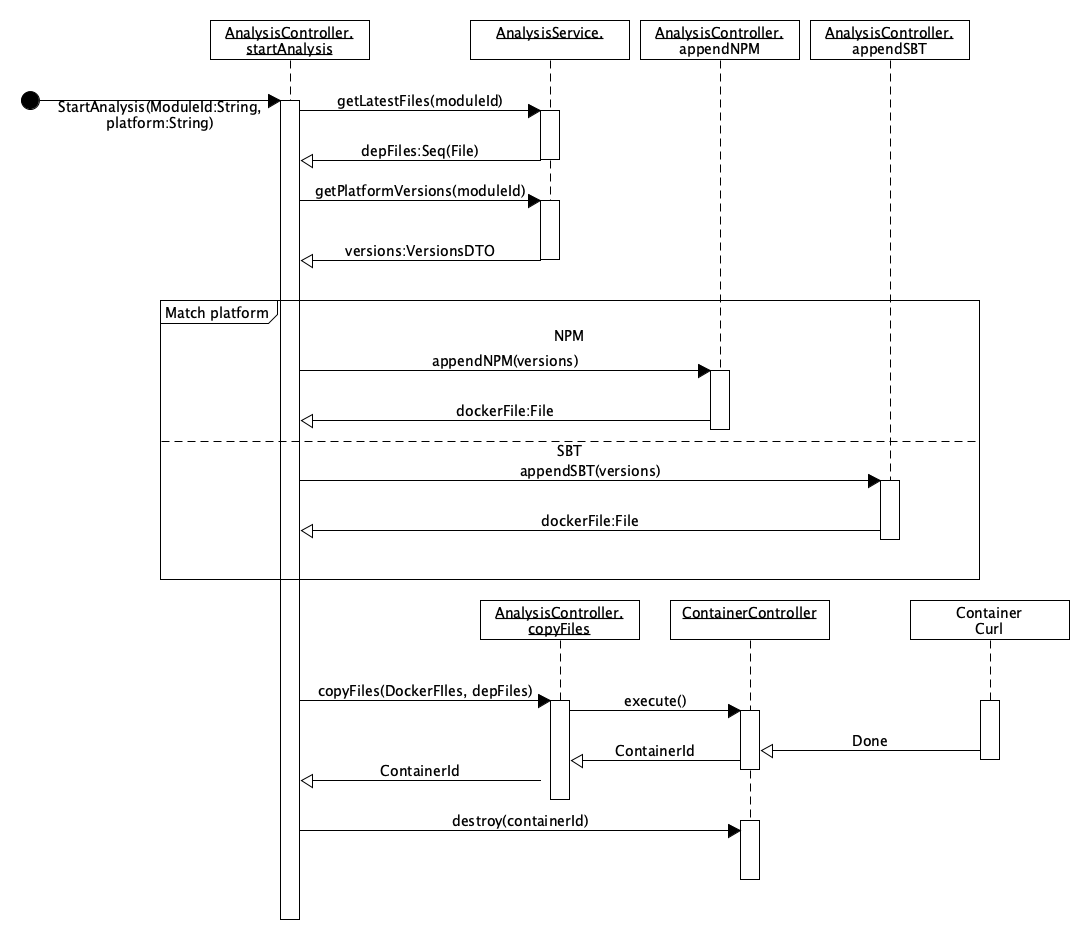
\includegraphics[width=10cm]{gfx/umlet/exports/PAE-CreateContainer}
    \caption{Componenten in de periodic Analysis Engine}
    \label{fig:paeSeq}
\end{figure}
In figuur ~\ref{fig:paeSeq} is te zien hoe een container wordt opgebouwd door middel van het aanmaken van een buildFile specifiek voor de module De buildfile is een build-file die in de JenkinsPipeline wordt gebruikt om een container aan te maken. om er zeker van te zijn worden de in de appendNPM/SBT stap de versies gecontroleerd en waar nodig aan gepast naar de nieuwere versies. Aan de buildfile worden nog commando's toegevoegd om de juiste dependency files toe tevoegen en het commando om de SCA Tool te runnen. Met als laatste stap de upload van het rapport en meta data naar de SOUPAPI zodat deze wordt genalyseerd. Op het moment dat deze upload succesvol is wordt de container vernietigd en de gebruikte bestanden verwijderd.
%
%\begin{figure}[bth]
%    \myfloatalign
%    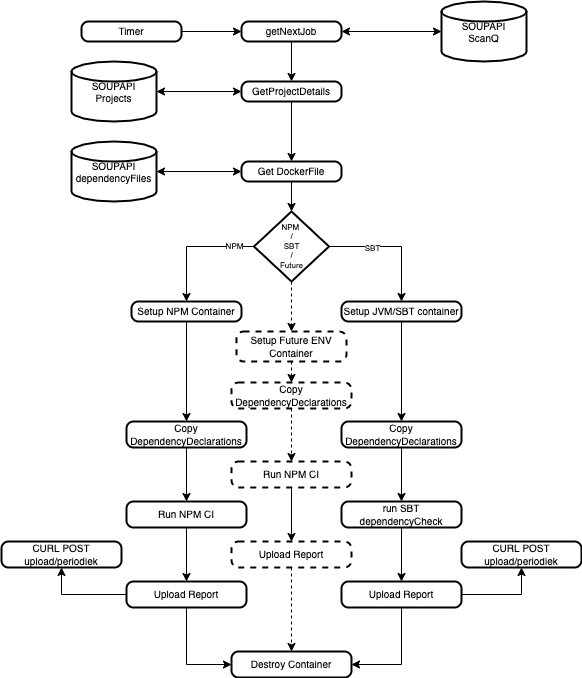
\includegraphics[width=15cm]{gfx/SOUPAPI-Periodic Analysis}
%    \caption{Periodieke analyse flow}
%    \label{fig:PeriodicAnalysis}
%\end{figure}

\subsection{AnalysisService}\label{subsec:analysisservice}
Deze service heeft een ondersteunende rol die het mogelijk maakt voor de controller om gegevens uit de API te kunnen halen die het nodig heeft om  zijn taken uit te kunnen voeren. Ook al lijkt deze service overbodig de reden dat er een extra service tussen zit is dat op het moment er in de api iets aangepast wordt er maar een enkele aanpassing nodig is in de service en niet op meerdere andere plekkem

\subsection{ScanQ en worklijst}\label{subsec:scanq}
In de database wordt een los tabel opgenomen met de in figuur~\ref{fig:scanQERD} weergeven attribuuten. Waarbij de lastAnalysis en nextAnalysis belangrijk zijn voor het schedulen van de jobs in de worklist.
De workList zelf is een interne lijst van de controller welke de voor die sessie resterende jobs bevat. Op het moment dat de controller klaar is met de analyses wordt de datum van lastAnalysis gezet op de datum van de analyse en de nextAnalysis op de datum van de volgede analyse welke ingesteld kan worden middels de projectsettings in de API database.
\begin{figure}[bth]
    \myfloatalign
    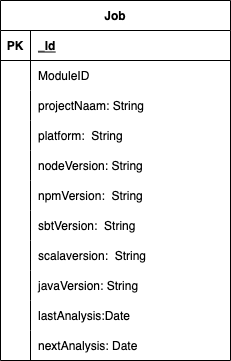
\includegraphics[width=5cm]{gfx/SOUPAPI-scanQERD}
    \caption{Table voor opslaan van Job in ScanQ}
    \label{fig:scanQERD}
\end{figure}
